% !TeX document-id = {b5392a94-51a3-49d1-9ba5-698bc09f9d35}
% !TeX encoding = UTF-8
% !TeX spellcheck = en_US
% !TeX TXS-program:bibliography = biber -l zh__pinyin --output-safechars %

\documentclass[a4paper,10pt]{article}

% to be `\input` in subfolders,
% ... therefore the path should be relative to subfolders.

\usepackage{iftex}
\ifPDFTeX
\else
	\usepackage[UTF8
		,heading=false
		,scheme=plain % English Document
	]{ctex}
\fi
%\ctexset{autoindent=true}
\usepackage{indentfirst}

\input{../.modules/basics/macros.tex}
\input{../.modules/preamble_base.tex}
\input{../.modules/preamble_beamer.tex}
\input{../.modules/basics/biblatex.tex}


%Misc
	\usepackage{lilyglyphs}
	\newcommand{\indicator}{$\text{\clefG}$}
	\newcommand{\indicatorInline}{$\text{\clefGInline}$}

\newcommand{\legacyReference}{{
%	\clearpage\par
%	\quad\clearpage
	\def{\midquote}{\textbf{PAST WORK, AS TEMPLATE}}
	\newparagraph
}}

% Settings
\counterwithout{equation}{section}
\mathtoolsset{showonlyrefs=false}
%\DeclareTextFontCommand{\textbf}{\sffamily}

% Spacing
\geometry{footnotesep=2\baselineskip} % pre footnote split
\setlength{\parskip}{.5\baselineskip}
\renewcommand{\baselinestretch}{1.15}


%% List
%	\setlist*{
%		listparindent=\parindent
%		,labelindent=\parindent
%		,parsep=\parskip
%		,itemsep=1.2\parskip
%	}


\addtobeamertemplate{navigation symbols}{}{%
    \usebeamerfont{footline}%
%    \usebeamercolor[fg]{footline}%
    \hspace{1em}%
    \large\insertframenumber/\inserttotalframenumber
}

\makeatletter
\setbeamertemplate{headline}
{%
    \begin{beamercolorbox}[wd=\paperwidth,colsep=1.5pt]{upper separation line head}
    \end{beamercolorbox}
    \begin{beamercolorbox}[wd=\paperwidth,ht=2.5ex,dp=1.125ex,%
      leftskip=.3cm,rightskip=.3cm plus1fil]{title in head/foot}
      \usebeamerfont{title in head/foot}\insertshorttitle
    \end{beamercolorbox}
    \begin{beamercolorbox}[wd=\paperwidth,ht=2.5ex,dp=1.125ex,%
      leftskip=.3cm,rightskip=.3cm plus1fil]{section in head/foot}
      \usebeamerfont{section in head/foot}%
      \ifbeamer@tree@showhooks
        \setbox\beamer@tempbox=\hbox{\insertsectionhead}%
        \ifdim\wd\beamer@tempbox>1pt%
          \hskip2pt\raise1.9pt\hbox{\vrule width0.4pt height1.875ex\vrule width 5pt height0.4pt}%
          \hskip1pt%
        \fi%
      \else%  
        \hskip6pt%
      \fi%
      \insertsectionhead
    \end{beamercolorbox}
% Code for subsections removed here
}
\makeatother
\input{../.modules/basics/biblatex.tex}

\title{A Modern Take on Renormalization}
%\addbibresource{.bib}

%%% ID: sensitive, do NOT publish!
%\InputIfFileExists{../id.tex}{}{}

\usepackage{cancel}

\begin{document}
\maketitle
\pagestyle{headings}
\pagenumbering{arabic}
\thispagestyle{empty}

\vspace*{-.5\baselineskip}
	The continuum limit $\Lambda\to\infty$ is \textbf{not} well defined.
	Renormalization provides a way to \emph{define} the theory when
	$\Lambda\to\infty$.
	
	\textbf{My belief:} The only way to fully understand renormalization is
	through Wilson's arguments; all other ``interpretations'' of
	renormalization are only \emph{heuristic}.

\textbf{Key words:}
\begin{itemize}[nosep]
\item Renormalization group
\item Counterterms
\item Regularization and cutoff
\end{itemize}


\setlength{\parskip}{.1\baselineskip}
\tableofcontents
\setlength{\parskip}{\parskipnorm}


\section{References}

\noindent \textsl{Ranked by importance:}

	\begin{itemize}
	\item David Skinner's note:
	  \begin{itemize}[nosep]
	  \item \url{https://www.damtp.cam.ac.uk/user/dbs26/AQFT.html}
	    \begin{itemize}[nosep]
	    \item \url{https://www.damtp.cam.ac.uk/user/dbs26/AQFT/Wilsonchap.pdf}
	    \item \url{https://www.damtp.cam.ac.uk/user/dbs26/AQFT/chap5.pdf}
	    \end{itemize}
	  \end{itemize}
	\item Schwartz, Chapter 15
	\item Peskin \& Schroeder, Chapter 10 \& 12
	\item Hollowood's book:
	  \begin{itemize}[nosep]
	  \item \url{https://arxiv.org/abs/0909.0859}
	  \item \url{https://link.springer.com/book/10.1007/978-3-642-36312-2}
	  \end{itemize}
	\end{itemize}

\section{Wilson's picture}
	Seed theory parameters (i.e.\ \emph{bare parameters}):
	$(g_0,\Lambda_0)$, $g = (m,\lambda,\cdots)$ a collection of all
	possible couplings.
	
	\begin{equation}
	\begin{aligned}
	  \phi_{\Lambda_0}(x)
	  \sim \int^{\Lambda_0} \dd p
	    e^{ip\cdot x}
	    \tilde{\phi}(p)
	  &= \int^{\Lambda} \dd p
	    e^{ip\cdot x}
	    \tilde{\phi}(p)
	    + \int_{\Lambda}^{\Lambda_0} \dd p
	    e^{ip\cdot x}
	    \tilde{\phi}(p) \\
	  &=\colon \phi_{\Lambda}(x) + \chi(x)
	\end{aligned}
	\end{equation}
	
	\begin{equation}
	\begin{aligned}
	  \DD\phi_{\Lambda_0}(x)
	  \sim \prod_{\norm{p} < \Lambda_0}
	    \dd{\tilde{\phi}(p)}
	  &= \prod_{\norm{p} < \Lambda}
	    \dd{\tilde{\phi}(p)}
	    \prod_{\Lambda < \norm{p} < \Lambda_0}
	    \dd{\tilde{\phi}(p)} \\
	  &\sim
	    \DD\phi_{\Lambda}(x)\,
	    \DD\chi(x)
	\end{aligned}
	\end{equation}
	
	\begin{equation}
	\begin{aligned}
	  \mcal{Z} (g_0,\Lambda_0)
	  &= \int \DD \phi_{\Lambda_0}
	      e^{iS[\phi_{\Lambda_0}]} \\
	  &= \int \DD \phi_{\Lambda}
	    \int \DD \chi\,
	      e^{iS[\phi_\Lambda + \chi]} \\
	  &=\colon \int \DD \phi_{\Lambda}\,
	      e^{iS_{\mathrm{eff}} [\phi_\Lambda]}
	  =\colon \mcal{Z}\pqty{g(\Lambda),\Lambda}
	\end{aligned}
	\end{equation}
	Renormalized parameters: $(g,\Lambda)$.
	
	\begin{quote}
	\textbf{Subtlety:} the notation above is only schematic; in practice we
	first Wick-rotate to Euclidean signature, so that the momentum cutoff is
	easily imposed: $\norm{p} = \sqrt{p_0^2 + \vb{p}^2} < \Lambda$. In
	Lorentzian signature, it's hard to define a covariant cutoff since
	$p_\mu p^\mu = - p_0^2 + \vb{p}^2$. This process can be made rigorous;
	just think of the 8-shaped contour in loop integrals.
	\end{quote}
	
	\textbf{Effective action:}
	\begin{equation}
	  S_{\mathrm{eff}}[\phi]
	  = -i \ln \int \DD \chi
	      e^{iS[\phi + \chi]} \\
	\end{equation}
	$\phi = \phi_\Lambda$ is treated as constant when doing
	$\int \DD \chi$.
	\begin{equation}
	\begin{aligned}
	  \mcal{L}[\phi + \chi]
	  &= - \frac{1}{2}
	      \partial_\mu (\phi + \chi)\,
	      \partial^\mu (\phi + \chi)
	    - \frac{1}{2} m^2
	      (\phi + \chi)^2
	    - \frac{1}{4!} \lambda\,
	      (\phi + \chi)^4\\
	  &= \cdots \\
	  &= \mcal{L}[\phi]
	    + \Delta\mcal{L} [\phi,\chi]
	\end{aligned}
	\end{equation}
	
	\begin{equation}
	  S_{\mathrm{eff}}[\phi_\Lambda]
	  = S[\phi_\Lambda]
	    - i \ln \int \DD \chi
	      e^{i\,\Delta S[\phi_\Lambda + \chi]} \\
	\end{equation}
	
	If $\Lambda \lesssim \Lambda_0$, then $S_{\mathrm{eff}}$ is almost
	the same as the original $S$, with minor corrections from the
	$\int \DD\chi$ term. Note that in our regularization scheme there will
	be no mixed terms of $\phi$ and $\chi$ in the effective action,
	since they have orthogonal Fourier modes.
	
	Note that $\mcal{Z}$ clearly does not depend on the intermediate scale $\Lambda$, we have:
	\begin{equation}
	  0
	  = \Lambda \dv{}{\Lambda}\,
	    \mcal{Z}\pqty{g(\Lambda),\Lambda}
	  = \pqty{
	      \Lambda \pdv{}{\Lambda}
	      + \Lambda \pdv{g^{(i)}}{\Lambda}
	        \pdv{}{g^{(i)}}
	    }
	    \mcal{Z}\pqty{g(\Lambda),\Lambda}
	\end{equation}
	This is an example of a \textbf{RG Equation}.
\section{Perturbative Renormalization}
	However, in naïve perturbation theory, we wish to complete the entire
	path integral $\mcal{Z} (g_0,\Lambda_0)$. We can think of this as
	integrating out more and more high energy modes, until we reach the IR
	scale $\Lambda \to 0$.
	
	When $\Lambda \ll \Lambda_0$, we have no reason to believe the
	renormalized couplings $g(\Lambda)$ are close to the original
	couplings $g_0$ at $\Lambda_0$. In fact, they may differ by a large
	(but finite) renormalization factor $Z$: $g_0 = Zg$.
	
\subsection{Counterterms}
	In the above analysis, the theory flows from UV to IR. However, in
	reality, the IR results are known from experiments, and we are trying to
	\emph{extrapolates} from IR to UV.
	
	We achieve this by \emph{tuning} the bare parameters $(g_0,\Lambda_0)$
	so that after RG flow, the IR results fit our experimental observations.
	If the IR couplings $g(\Lambda)$ are finite and small, then since
	$\Lambda \ll \Lambda_0$, we expect $g_0$ to be very large.
	
	We often \emph{split} $g_0$ into 2 parts for convenience:
	\begin{equation}
	  g_0 = g + \var{g}
	  = g + (Z - 1)\,g
	\end{equation}
	$\var{g}$ is the so-called \emph{counterterm}; intuitively, it's the
	(large) correction that gets integrated out when we go from
	$\Lambda_0$ all the way to IR.
	
	Basically, we have the following procedure:
	
	\begin{figure}[!h]
	\centering
	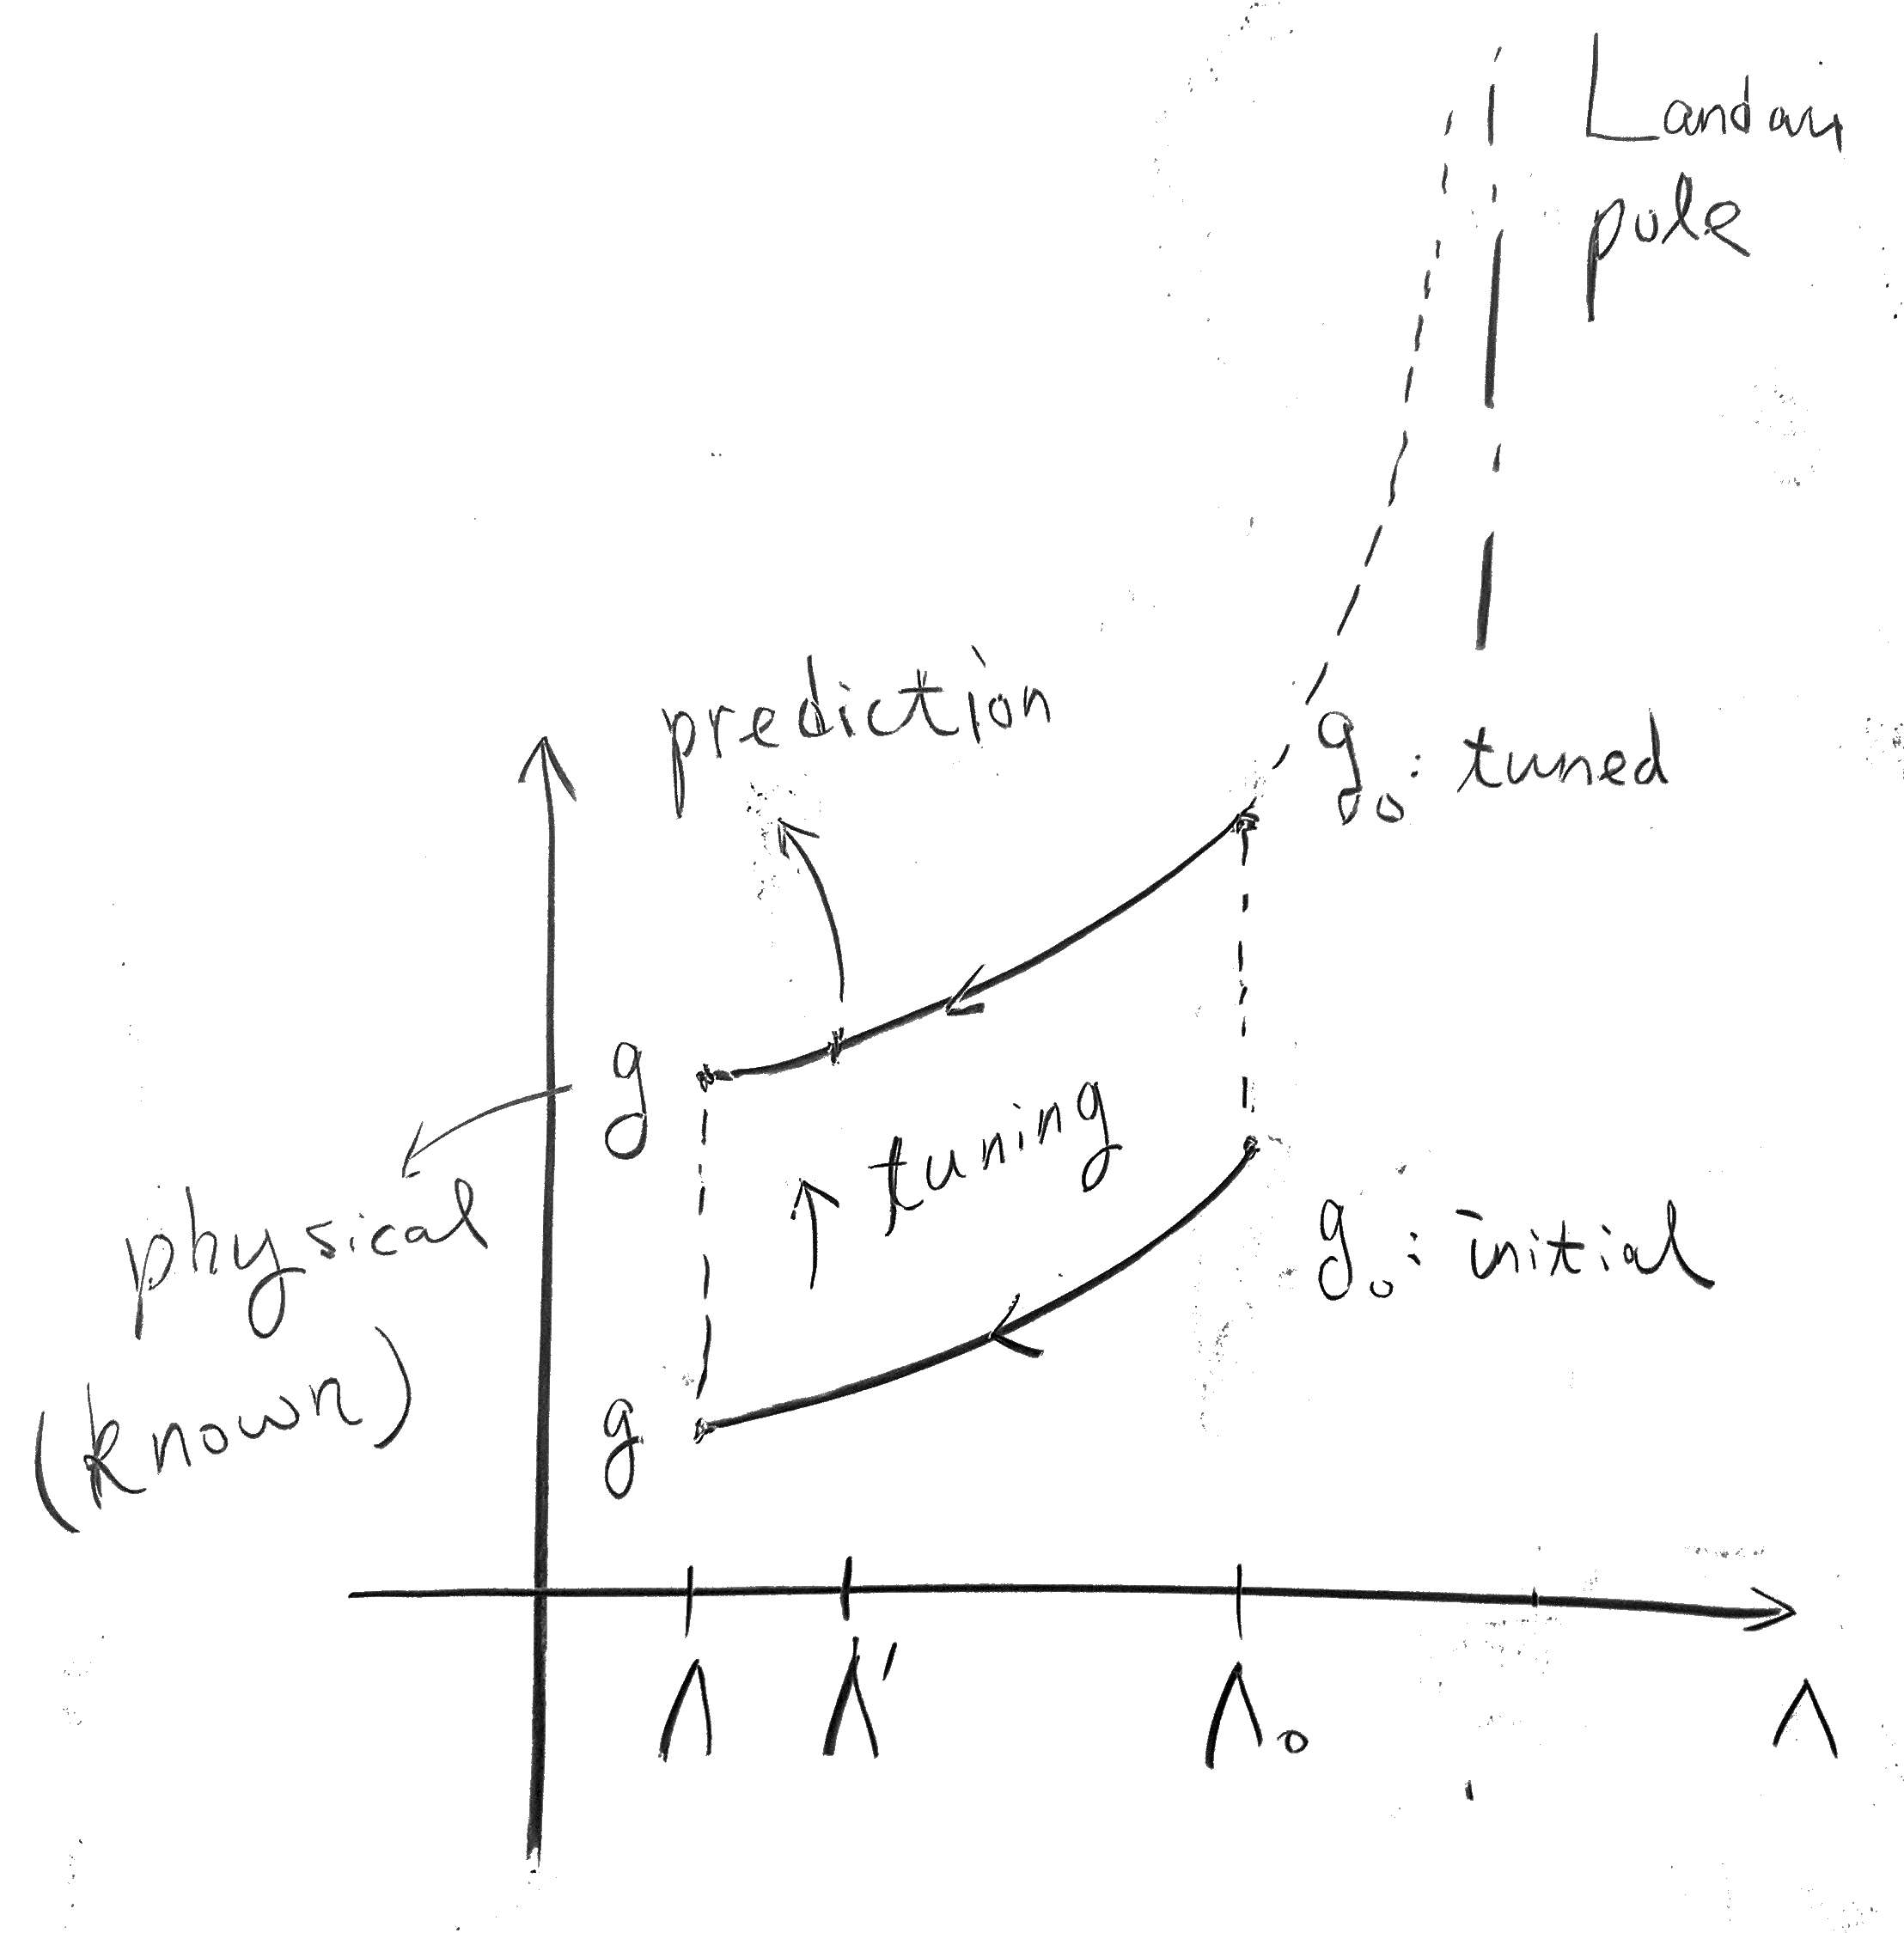
\includegraphics[width=.5\linewidth]{img/RG-process.png}
	\end{figure}
	
	\begin{enumerate}[noitemsep,midpenalty=100]
	\setcounter{enumi}{-1}
	
	\item
	  Select some UV parameters $(g_0,\Lambda_0)$
	\item
	  Perform the RG flow: $(g_0,\Lambda_0)\to (g,\Lambda)$
	\item
	  Tune (redefine) $g_0$ so that $(g,\Lambda)$ matches with
	  experiments
	\item
	  Use the tuned data to predicts phenomena at a different scale
	  $(g',\Lambda')$
	\end{enumerate}
	
	Note that the tuning of UV parameters $g_0$ is \emph{far from unique!}
	This is easy to understand: many UV theories might flow to the same IR
	theory. For this reason, some would say that RG is a \emph{semi-group}.
	
	However, for a \emph{renormalizable} theory, we can restrict the tuning
	to a \emph{finite} dimensional subspace formed by the \emph{relevant}
	couplings, since most other parameters $g^{(i)}$ are \emph{irrelevant}
	and get suppressed by $\Lambda/\Lambda_0$ in the IR. After such
	restriction to a relevant subspace, the RG flow is a group, and we can
	reverse the flow to \emph{extrapolate} towards UV.
	

\subsection{Perturbation}
	
	The above results are non-perturbative and should always hold.
	Perturbation theory is only a way to calculate the RG flow from UV to
	IR; it is reliable only if the IR coupling $g$ is sufficiently small.
	In this case we can tune $(g_0,\Lambda_0)$ with the following
	recursive / iterative algorithm:
	
	\begin{enumerate}[noitemsep]
	\item
	  Perturbative calculation of RG flow:
	  $(g_0,\Lambda_0)\to (g,\Lambda)$ at $\order{g^n}$
	\item
	  Tune (redefine) $(g_0,\Lambda_0)$ by adding counterterms, so that
	  $(g,\Lambda)$ matches with experiments
	\item
	  Increase order $n$ and go to step 1
	\end{enumerate}
	
	The (non-)renormalizability of a theory is evident in the perturbative
	expansion, by counting the \textbf{superficial degrees of divergence}
	$D$ of the Feynman diagrams. Basically,
	
	\begin{itemize}
	\item
	  Interaction vertices create loops, and loops create UV divergences.
	  Higher order interaction vertices create more loops, which lead to
	  more divergences.
	\item
	  External lines suppress UV divergences by factors like
	  $\frac{1}{\cancel{p}}$ or $\frac{1}{p^2}$.
	\end{itemize}
	
	For a renormalizable theory, there will be no divergence for diagrams
	with a sufficient number $E$ of external legs; for a
	non-renormalizable theory, however, there will always be divergences, no
	matter how large $E$ is.
	
\subsection{Renormalization Schemes}
	
	There is a subtlety in the above procedure: how do we actually relate IR
	parameters $(g,\Lambda)$ with actual physical quantities,
	e.g.~amplitudes $\mcal{M}(\mu)$?
	
	In fact, we've assumed that $(g,\Lambda)_{\Lambda\to 0}$ gives the
	physical couplings that we are familiar with, e.g.~mass, electric charge
	and so on. This is not quite true, since physical quantities are
	actually defined with scattering amplitudes. There are different choices
	of relating $g$ with physical observables; this lead to various
	renormalization schemes:
	
	\begin{itemize}[nosep]
	
	\item
	  On-shell / pole-mass scheme
	\item
	  Minimal subtraction ($\mathrm{MS}$) \& modified MS
	  ($\overline{\mathrm{MS}}$)
	\end{itemize}
	
	\hypertarget{renormalizability}{%
	\section{Renormalizability}\label{renormalizability}}
	
	Most parameters $g^{(i)}$ are, in fact, \emph{irrelevant} --- such
	terms in the Lagrangian get suppressed by $\Lambda/\Lambda_0$ in IR.
	If the IR theory has only \emph{relevant} couplings, then one should be
	able to recover their physical values by tuning a finite amount of
	relevant couplings in the UV, and usually the tuning is unique. This is
	the defining characteristic of a \textbf{renormalizable} theory.
	Basically, this means that we can naturally obtain a UV theory by
	extrapolation.
	
	\begin{quote}
	However, the tuning process described above might encounter some serious
	obstruction: the tuned $g_0$ could blow up at some finite
	$\Lambda_{\mathrm{UV}}$; this is the so-called \emph{Landau pole}.
	This tells us that the theory only works under some
	$\Lambda_{\mathrm{UV}}$, i.e.~it is not \emph{UV complete}; it's only
	an \emph{effective} theory. One have to ``embed'' this Lagrangian into a
	bigger theory that works beyond $\Lambda_{\mathrm{UV}}$; this is the
	non-trivial \emph{UV completion} of an effective theory.
	\end{quote}
	
	On the other hand, a theory is \textbf{non-renormalizable} if it
	contains irrelevant couplings in the IR. In this case the IR parameters
	$g$ depend sensitively on small perturbations of the UV parameters
	$g_0$, and one has to tune infinitely many bare parameters to obtain
	the physical IR values. Such theory is hardly \emph{fundamental}, since
	it depends on infinitely many parameters; but it's a good
	\emph{effective theory} nonetheless.
	
\section{Effective Action}
	
	Furthermore, after $\phi_\Lambda$ is completely integrated out, we
	have:
	
	\begin{equation}
	  S_{\mathrm{eff}}[\phi] \to W,\quad
	  Z(g_0,\Lambda_0) = e^{iW}
	\end{equation}
	Note that $W$ no longer has any $\phi$ dependence, but it is a
	function of $(g_0,\Lambda_0)$, which in turn is tuned by physical
	$(g,\Lambda)$. $W$ in fact contains all information about the seed
	theory, labeled by $(g_0,\Lambda_0)$. To extract this information, we
	usually perturb the original action $S[\phi]$ with a source term; then
	we have:
	
	\begin{equation}
	  S[\phi,J]
	  = S[\phi] + \int \dd{x}\,J(x)\,\phi(x),\quad
	  W \to W[J]
	\end{equation}
	
	Expand $W[J]$ in terms of $J$-modes, and its coefficient gives us
	physical coupling constants in the IR. More precisely, we can define the Legendre-transformed $\Gamma[\varphi]$.


\printbibliography[%
%	title = {参考文献} %
	,heading = bibintoc
]
\end{document}
